\chapter{TINJAUAN PUSTAKA}
\label{chap:tinjauanpustaka}

% Ubah bagian-bagian berikut dengan isi dari tinjauan pustaka

Demi mendukung penelitian ini, dibutuhkan beberapa \textit{state of the art} dan teori penunjang sebagai bahan acuan dan referensi. Dengan demikian penelitian ini menjadi lebih terarah.

\section{\textit{State of The Art}}
\label{penelitianterkait}

\subsection{Real-Time Pedestrian Detection With Deep Network Cascades}
\label{realtime-pedestrian}

Penelitian ini dilakukan oleh Anelia Angelova dan kawan-kawan pada tahun 2015 yang menyajikan pendekatan \textit{real-time} baru untuk deteksi objek yang mengeksploitasi efisiensi \textit{cascade classifiers} dengan akurasi \textit{deep neural network} \citep{penelitianterkait1}. \textit{Deep network} telah terbukti unggul dalam tugas klasifikasi, dan kemampuannya untuk beroperasi pada \textit{raw pixel input} tanpa perlu merancang fitur khusus. Namun, \textit{deep network} terkenal lambat pada waktu inferensi. Dalam \textit{paper} tersebut, Anelia Angelova dan kawan-kawan mengusulkan pendekatan \textit{cascades deep network} dan \textit{fast features}, yang sangat cepat dan sangat akurat. Mereka menerapkannya pada permasalahan pada deteksi pejalan kaki. Algoritma mereka berjalan secara \textit{real-time} pada 15 \textit{frame} per detik. Pendekatan yang dihasilkan mencapai tingkat kesalahan rata-rata 26,2\% pada \textit{benchmark} deteksi Caltech Pedestrian.

\subsection{Pedestrian Detection: The Elephant In The Room}
\label{pedestrian-detection}

Deteksi pejalan kaki digunakan di banyak aplikasi berbasis citra mulai dari pengawasan video hingga pengemudi otonom. Meskipun mencapai kinerja tinggi, sebagian besar masih belum diketahui seberapa baik detektor yang ada menggeneralisasi data yang tidak terlihat. Hal ini penting karena detektor yang praktis harus siap digunakan dalam berbagai skenario dalam aplikasi. Untuk tujuan tersebut, Irtiza Hasan dan kawan-kawan melakukan studi komprehensif dalam \textit{paper} ini, menggunakan prinsip umum evaluasi \textit{cross-dataset} langsung \citep{pedestrian-detection}. Melalui \textit{paper} ini, ditemukan bahwa detektor pejalan kaki terkini yang ada, meskipun berkinerja cukup baik ketika dilatih dan diuji pada kumpulan data yang sama, namun secara umum memiliki peforma yang cukup buruk dalam evaluasi \textit{cross-dataset}. 

Dalam \textit{paper} ini ditunjukkan bahwa ada dua alasan untuk permasalahan ini. Pertama, desain yang dibuat (misalnya, \textit{anchor settings}) mungkin bias terhadap tolok ukur dalam \textit{training} dan \textit{test pipeline} data tunggal, tetapi akibatnya sebagian besar membatasi kemampuan generalisasi dari keduanya. Kedua, sumber pelatihan umumnya tidak terlalu padat pada pejalan kaki dan mempunyi beragam dalam skenario. Di dalam evaluasi \textit{cross-dataset} langsung, secara mengejutkan, ditemukan bahwa detektor objek dengan tujuan umum, tanpa adaptasi khusus untuk pejalan kaki dalam desain, digeneralisasi jauh lebih baik dibandingkan dengan detektor pejalan kaki terkini yang ada. Lebih lanjut, diilustrasikan bahwa kumpulan data yang beragam dan padat, yang dikumpulkan dengan \textit{crawling web} , berfungsi sebagai sumber pra-pelatihan yang efisien untuk deteksi pejalan kaki. Oleh karena itu, pada \textit{paper} mengusulkan \textit{training pipelin} progresif dan menemukan bahwa \textit{pipeline} tersebut berfungsi dengan baik untuk deteksi pejalan kaki yang berorientasi pada pengemudian otonom. Akibatnya, studi yang dilakukan dalam makalah ini menunjukkan bahwa lebih banyak penekanan harus diberikan pada evaluasi \textit{cross-datasset} untuk desain masa mendatang pada detektor pejalan kaki.

\subsection{Fast Vehicle and Pedestrian Detection Using Improved Mask R-CNN}
\label{fast-vehicle}

Penelitian ini menyajikan algoritma Mask R-CNN yang sederhana dan efektif untuk deteksi kendaraan dan pejalan kaki yang lebih cepat \citep{fast-vehicle}. Metode ini memiliki nilai praktis untuk sistem peringatan anti-tabrakan dalam mengemudi cerdas. \textit{Deep Neural Network} dengan lebih banyak lapisan memiliki kapasitas yang lebih besar, tetapi juga harus melakukan perhitungan yang lebih rumit. Untuk mengatasi kelemahan ini, penelitian ini mengadopsi jaringan Resnet-86 sebagai \textit{backbone} yang berbeda dari struktur tulang punggung Resnet-101 dalam algoritma Mask R-CNN. Hasilnya menunjukkan bahwa jaringan Resnet-86 dapat mengurangi waktu operasi dan sangat meningkatkan akurasi. Kendaraan dan pejalan kaki yang terdeteksi juga disaring berdasarkan dataset Microsoft COCO. Dataset baru dibentuk dengan menyaring dan melengkapi COCO dataset, yang membuat pelatihan algoritma lebih efisien. Bagian terpenting dari penelitian ini adalah diusulkannya algoritma baru, \textit{Side Fusion FPN}. Parameter dalam algoritma tidak ada perubahan, jumlah perhitungan meningkat kurang dari 0,000001, dan rata-rata presisi (mAP) meningkat 2,00 poin. Hasilnya menunjukkan bahwa, dibandingkan dengan algoritma Mask R-CNN, algoritma pada penelitian ini menurunkan ukuran memori bobot sebesar 9,43\%, meningkatkan kecepatan pelatihan sebesar 26,98\%, meningkatkan kecepatan pengujian sebesar 7,94\%, menurunkan nilai \textit{error} sebesar 0,26, dan meningkatkan nilai mAP sebesar 17,53 poin.

\subsection{MASK R-CNN for Pedestrian Crosswalk Detection and Instance Segmentation}
\label{pedestrian-crosswalk}

Pejalan kaki paling rentan mengalami kecelakaan mengingat mayoritas pengendara mengecualikan mereka sebagai pengguna jalan \citep{pedestrian-crosswalk}. Pada penelitian ini, pendeteksian objek menggunakan Mask Region-Based CNN dan segmentasi instance diterapkan pada penyeberangan pejalan kaki. Pelatihan dilakukan menggunakan Mask R-CNN untuk deteksi objek dengan backbone ResNet-101, dengan kecepatan pembelajaran 0,001 dan 2 gambar per GPU selama 30 epoch dari 100 batch. Berdasarkan penelitian ini, 500 gambar penyeberangan pejalan kaki dikumpulkan dan dipilih untuk validasi dan pelatihan. 80\% dari gambar adalah untuk set pelatihan dan untuk set validasi adalah 20\%. 30 gambar pengujian penyeberangan pejalan kaki lainnya dikumpulkan untuk evaluasi model guna memverifikasi stabilitas dan keandalan model yang terlatih. Semua 30 gambar pengujian telah terdeteksi dan akurasi deteksi lebih besar dari 97\%. Jika ada 2 atau lebih penyeberangan pejalan kaki dalam sebuah gambar, maka akan membuat warna MASK berbeda untuk setiap deteksi. Ringkasan hasil tes memverifikasi bahwa semua data yang dikumpulkan lebih tinggi dari 97\% untuk dapat mendeteksi pejalan kaki.

\section{Teori Penunjang}
\label{sec:dasarteori}


\subsection{\textit{Machine Learning}}
\label{subsec:machine-learning}

\textit{Machine Learning} adalah studi tentang algoritma komputer yang memberikan sistem kemampuan untuk belajar secara otomatis dan dapat meningkatkan kemampuan dari pengalaman yang sudah didapatkan \citep{machinelearning1}. Hal ini umumnya dilihat sebagai sub-bidang kecerdasan buatan. Algoritma pembelajaran mesin memungkinkan sistem membuat keputusan secara mandiri tanpa dukungan eksternal. Keputusan semacam itu dibuat dengan menemukan pola dasar yang berharga dalam data yang kompleks. Berdasarkan pendekatan pembelajaran, jenis data \textit{input} dan \textit{output}, dan jenis masalah yang dipecahkan, ada beberapa kategori utama dari algoritma \textit{machine learning} \textit{supervised, unsupervised} dan \textit{reinforcement learning}. Ada beberapa pendekatan hibrida dan metode umum lainnya yang menawarkan ekstrapolasi alami dari bentuk masalah pembelajaran mesin. Berikut merupakan penjelasan dari beberapa kategori utama dari algoritma \textit{machine learning}:

\begin{enumerate}
	\item \textit{Supervised Learning} diterapkan ketika data dalam bentuk variabel input dan nilai target output. Algoritma akan mempelajari fungsi pemetaan dari \textit{input} ke \textit{output}. Ketersediaan sampel data berlabel dengan skala besar mempunyai nilai yang tinggi dikarenakan masih terdapat kelangkaan \textit{dataset}. Pendekatan ini secara luas dapat dibagi menjadi dua kategori utama yaitu \textit{classification} dan \textit{regression}. Gambar \ref{fig:supervised} menampilkan visualisasi dari \textit{classification} dan \textit{regression} pada \textit{Supervised Learning}
	
	\begin{figure}[ht]
		\centering
		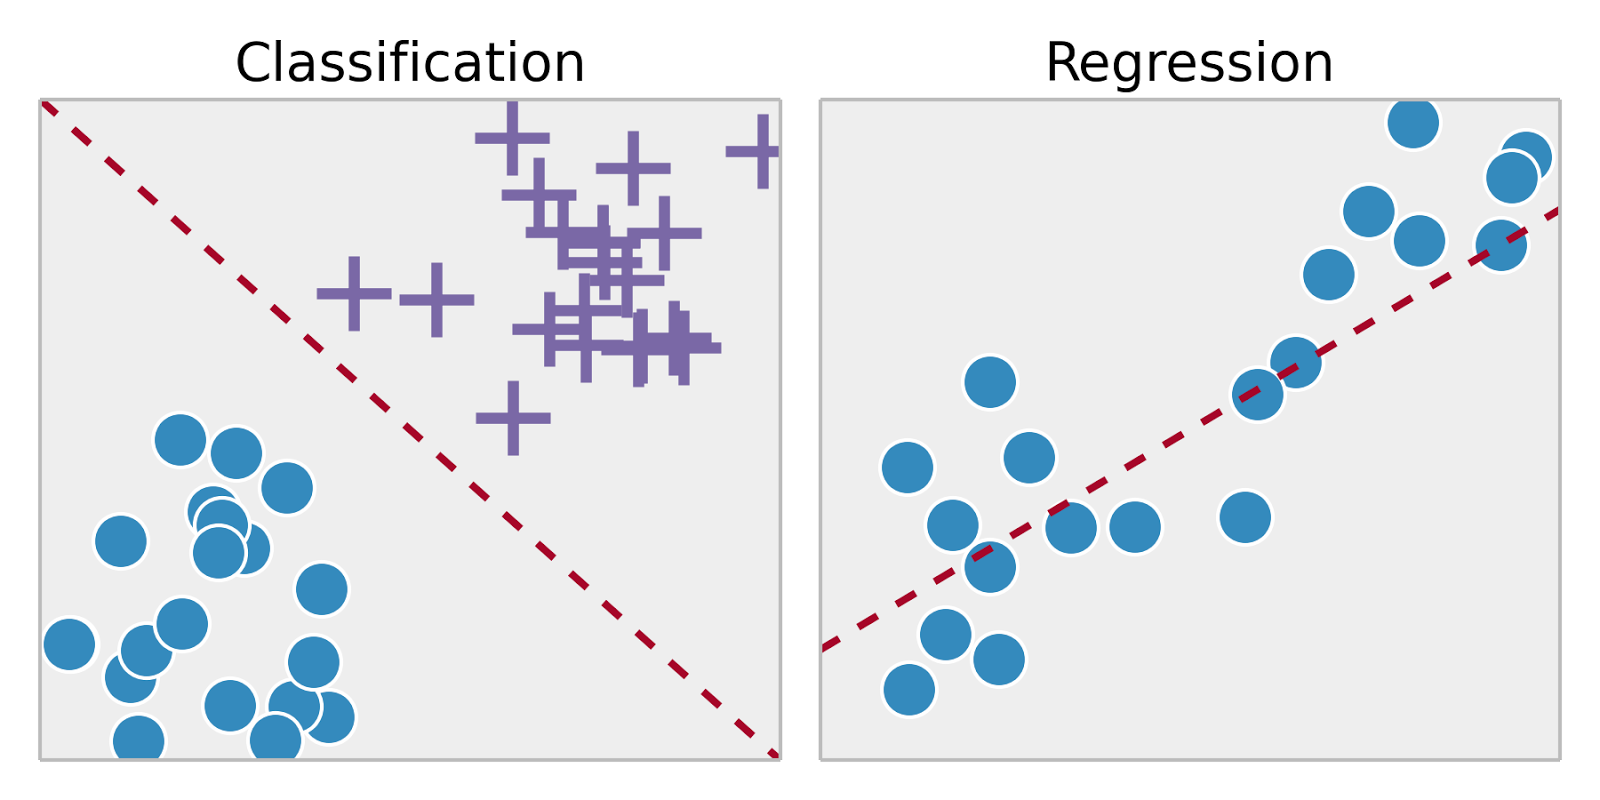
\includegraphics[scale=0.1]{gambar/supervised.png}
		\caption{Gambaran \textit{Supervised Learning}\citep{supervised}}
		\label{fig:supervised}
	\end{figure}  
	
	\item \textit{Unsupervised Learning} diterapkan ketika data hanya tersedia dalam bentuk \textit{input} dan tidak ada variabel \textit{output} yang sesuai. Algoritma semacam itu memodelkan pola yang mendasari data untuk mempelajari lebih lanjut tentang karakteristiknya. Salah satu jenis utama dari algoritma \textit{unsupervised} adalah pengelompokan. Dalam teknik ini, kelompok yang melekat dalam data ditemukan dan kemudian digunakan untuk memprediksi \textit{output} untuk \textit{input} yang tidak terlihat. Contoh dari teknik ini adalah untuk memprediksi perilaku pembelian pada pelanggan. Gambar \ref{fig:unsupervised} merupakan visualisasi dari algoritma \textit{unsupervised learning}.
	
	\begin{figure}[ht]
		\centering
		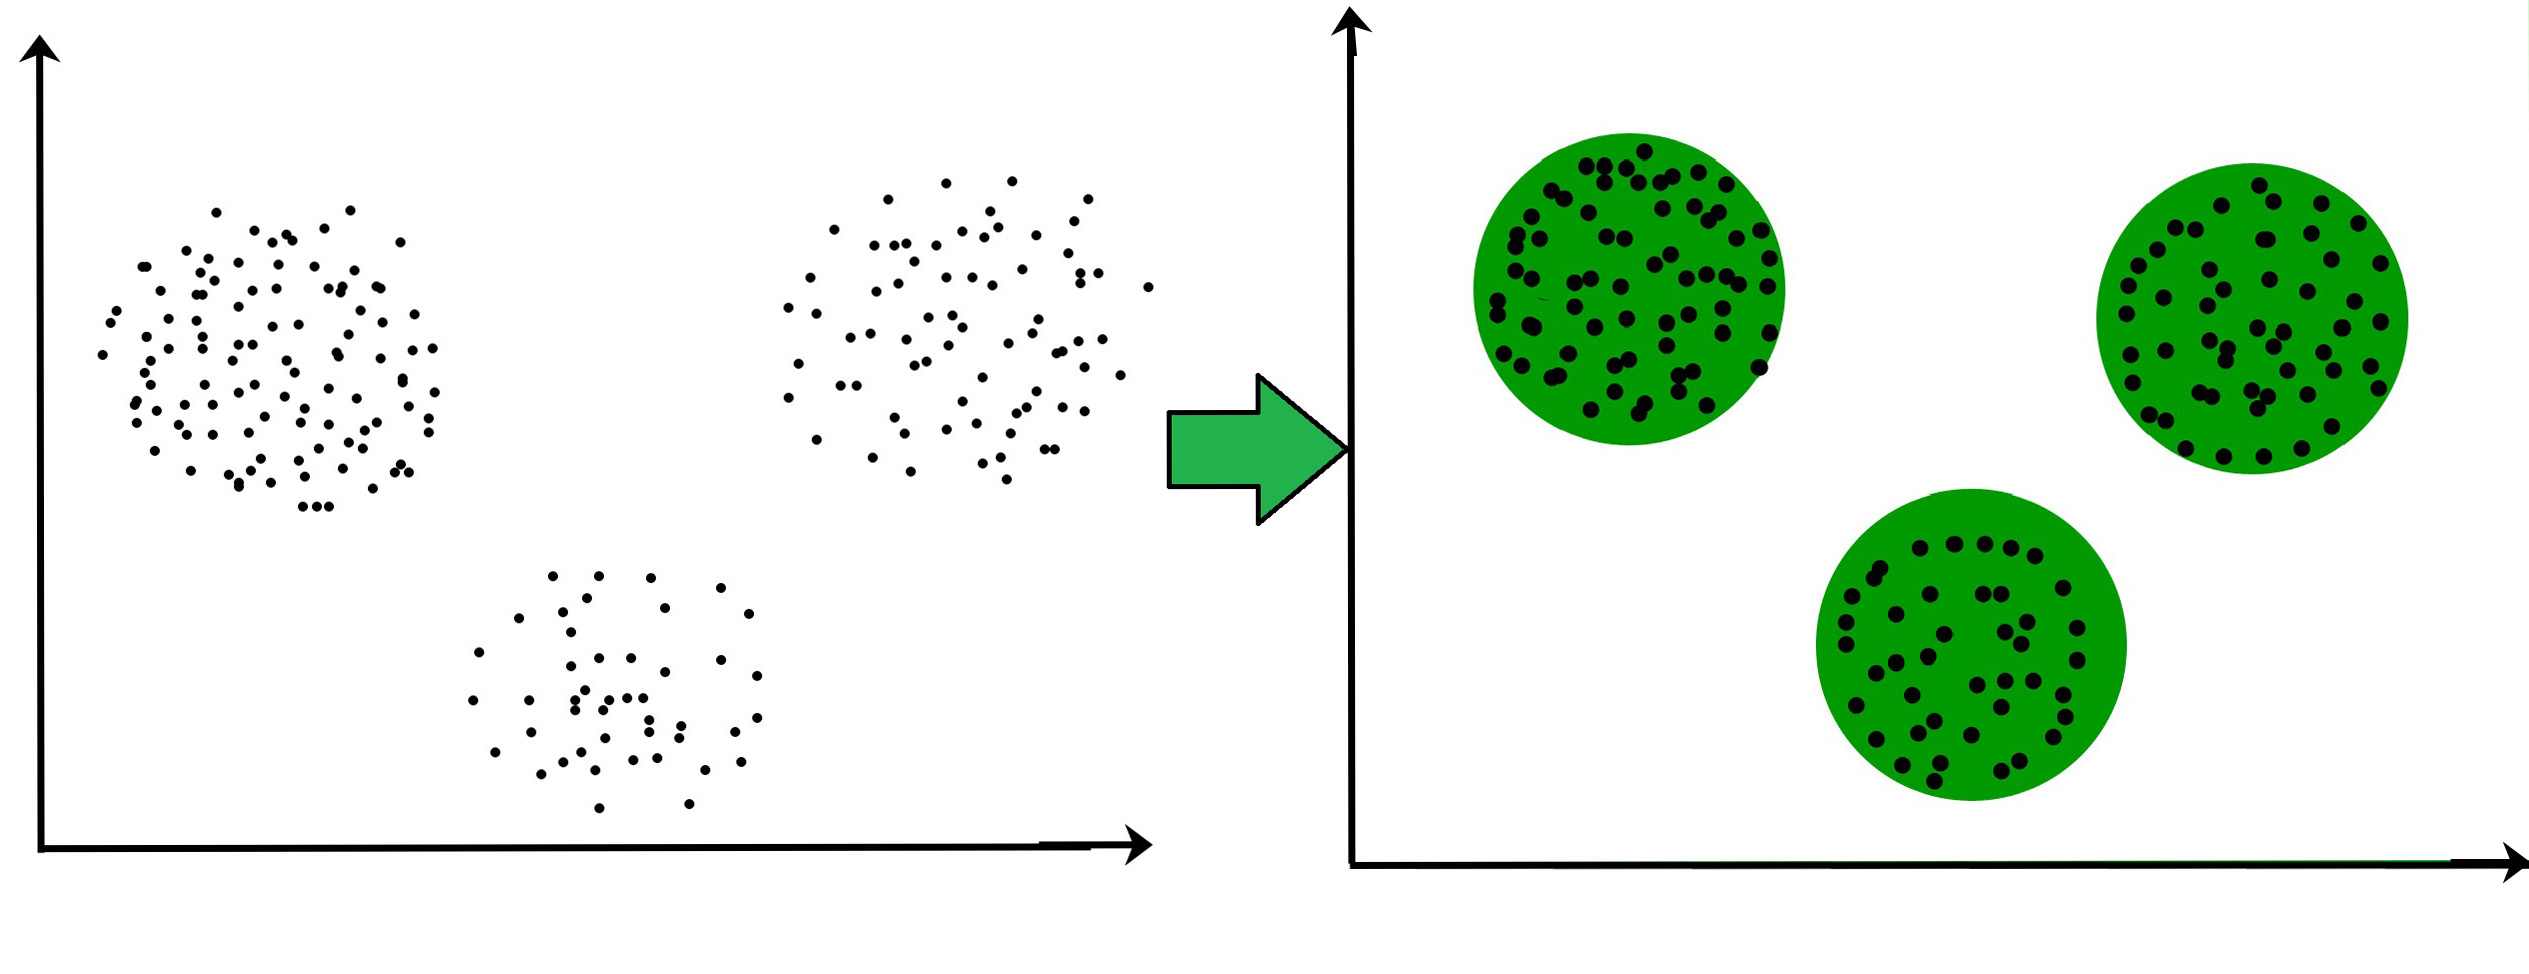
\includegraphics[scale=0.2]{gambar/unsupervised.jpg}
		\caption{Gambaran \textit{Unsupervised Learning}\citep{unsupervised}}
		\label{fig:unsupervised}
	\end{figure}
	
	
	\item \textit{Reinforcement learning} diterapkan ketika tugas yang ada
	adalah membuat urutan keputusan menuju \textit{reward} akhir. Selama proses \textit{learning}, \textit{artificial agent} mendapat \textit{reward} atau \textit{penalties} atas tindakan yang dilakukannya. Tujuannya adalah untuk memaksimalkan total \textit{reward} yang didapatkan. Gambar \ref{fig:reinforcement} merupakan visualisasi dari algoritma \textit{reinforcement learning}.
	
	\begin{figure}[ht]
		\centering
		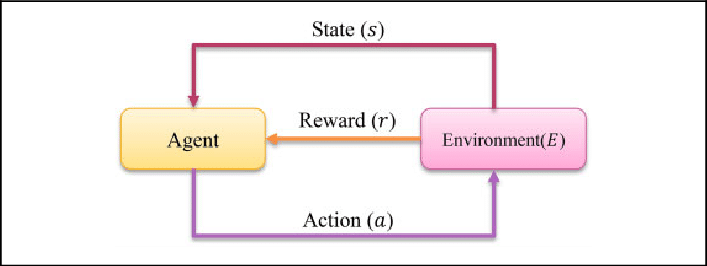
\includegraphics[scale=0.3]{gambar/reinforcement.png}
		\caption{Gambaran \textit{Reinforcement Learning}\citep{reinforcement}}
		\label{fig:reinforcement}
	\end{figure}
\end{enumerate}

\subsection{\textit{Deep Learning}}
\label{subsec:deeplearning}

\textit{Deep Learning} adalah kelas \textit{machine learning} yang berkinerja jauh lebih baik pada data tidak terstruktur\citep{dl}. Teknik \textit{deep learning} mengungguli teknik \textit{machine learning} saat ini. Ini memungkinkan model komputasi untuk mempelajari fitur secara progresif dari data di berbagai level. Popularitas \textit{deep learning} diperkuat karena jumlah data yang tersedia meningkat serta kemajuan perangkat keras yang menyediakan komputer yang kuat.

Arsitektur \textit{deep learning} berkinerja lebih baik daripada jaringan saraf tiruan  sederhana, meskipun waktu \textit{learning} dari struktur \textit{deep learning} lebih tinggi dari jaringan saraf tiruan. Namun, waktu \textit{learning} dapat dikurangi dengan menggunakan metode seperti \textit{transfer learning} atau komputasi menggunakan GPU. Salah satu faktor yang menentukan keberhasilan jaringan saraf terletak pada desain arsitektur jaringan yang cermat.

\subsection{\textit{Convolutional Neural Network}}
\label{subsec:cnn}

\textit{Convolutional Neural Networl} (CNN) adalah jenis khusus dari \textit{multilayer neural network} atau arsitektur \textit{deep learning} yang terinspirasi oleh sistem visual makhluk hidup \citep{cnn}. CNN sangat cocok untuk berbagai bidang visi komputer dan \textit{natural language processing}. \textit{Convolutional Neural Network} (CNN), juga disebut \textit{ConvNet}, adalah jenis \textit{Artificial Neural Network} (ANN), yang memiliki arsitektur \textit{feed-forward} yang dalam dan memiliki kemampuan generalisasi yang luar biasa dibandingkan dengan jaringan lain dengan lapisan FC (\textit{Fully Connected}), ia dapat mempelajari fitur objek yang sangat abstrak terutama data spasial dan dapat mengidentifikasinya dengan lebih efisien. Model CNN yang dalam terdiri dari satu set lapisan pemrosesan yang dapat mempelajari berbagai fitur data \textit{input} (misalnya gambar) dengan beberapa tingkat abstraksi seperti yang ditampilkan pada Gambar \ref{fig:concept-cnn}. Lapisan inisiator mempelajari dan mengekstrak fitur tingkat tinggi (dengan abstraksi yang lebih rendah), dan lapisan yang lebih dalam mempelajari dan mengekstrak fitur tingkat rendah (dengan abstraksi yang lebih tinggi).

\begin{figure}[ht]
	\centering
	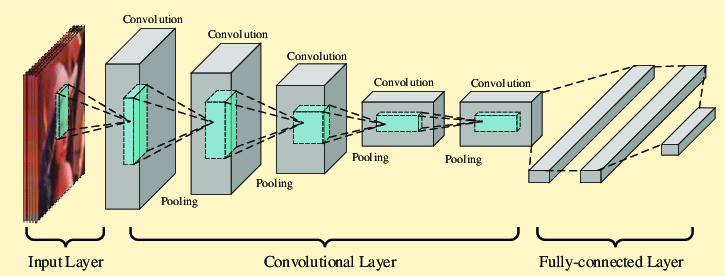
\includegraphics[scale=0.3]{gambar/concept-cnn.png}
	\caption{Gambaran Konsep Arsitektur CNN \citep{concept-cnn}}
	\label{fig:concept-cnn}
\end{figure}

\textit{Convolutional Neural Network} memiliki beberapa keunggulan dibanding dengan jaringan saraf tiruan lainnya dalam konteks visi komputer, antara lain :

\begin{enumerate}
	\item Salah satu alasan utama untuk mempertimbangkan CNN dalam kasus tersebut adalah fitur pembagian bobot dari CNN, yang mengurangi jumlah parameter yang dapat dilatih dalam jaringan, yang membantu model untuk menghindari \textit{overfitting} dan juga untuk meningkatkan generalisasi.
	\item Pada CNN, lapisan klasifikasi dan lapisan ekstraksi fitur melakukan proses \textit{learning} secara bersama-sama, yang membuat output model lebih terorganisir dan membuat output lebih bergantung pada fitur yang diekstraksi.
	\item Implementasi pada jaringan dengan ukuran yang besar akan lebih sulit dilakukan dengan menggunakan jenis jaringan saraf lain daripada menggunakan \textit{Convolutional Neural Network}
\end{enumerate}

\subsection{\textit{Regional-Based CNN}}
\label{subsec:rcnn}

Semenjak\textit{ Convolution Neural Network} (CNN) dengan \textit{fully connected layer} tidak mampu menangani frekuensi kemunculan dan multi objek. Salah satu cara untuk mengatasinya adalah dengan menggunakan \textit{sliding window brute force search} untuk memilih wilayah dan menerapkan model CNN pada area tersebut, tetapi masalah dari pendekatan ini adalah bahwa objek yang sama dapat direpresentasikan dalam gambar dengan ukuran dan aspek rasio yang berbeda. Dengan mempertimbangkan faktor-faktor tersebut, penerapan algoritma \textit{deep learning} (CNN) pada jumlah \textit{region proposal} yang banyak akan menyebabkan proses komputasi yang dijalankan akan menjadi sangat berat dan rumit.

\begin{figure}[h!]
	\centering
	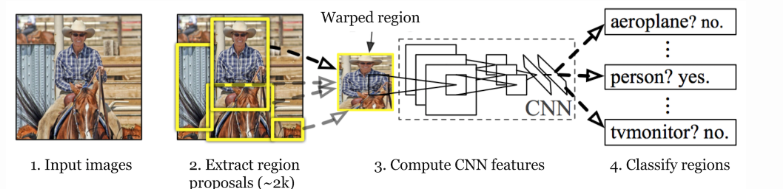
\includegraphics[scale=0.3]{gambar/rcnn.png}
	\caption{Arsitektur R-CNN \citep{arch-rcnn}}
	\label{fig:rcnn}
\end{figure}

Ross Girshick dan kawan-kawan pada tahun 2013 mengusulkan arsitektur baru yang disebut R-CNN seperti pada Gambar \ref{fig:rcnn} (\textit{Regional-based CNN}) untuk menghadapi tantangan deteksi objek ini \citep{rcnn}. Arsitektur R-CNN menggunakan algoritma \textit{selective search} yang menghasilkan sekitar 2000 \textit{region proposal}. \textit{Regional proposal} ini kemudian diterapkan ke arsitektur CNN untuk menghitung jumlah fitur CNN. Fitur-fitur ini kemudian diteruskan dalam model SVM untuk mengklasifikasikan objek yang ada di \textit{region proposal}. Langkah selanjutnya adalah melakukan regresi pada \textit{bounding box} untuk mengetahui lokasi objek yang ada dalam gambar dengan lebih tepat. 

\subsection{\textit{Fast R-CNN}}
\label{subsec:fast-rcnn}

Fast R-CNN ditemukan atas metode yang telah ditemukan terlebih dahulu yaitu \textit{R-CNN} untuk mengklasifikasikan proposal objek secara efisien menggunakan \textit{deep convolutional network} \citep{fast-rcnn}. Dibandingkan dengan \textit{R-CNN}, \textit{Fast R-CNN} menggunakan beberapa inovasi untuk meningkatkan kecepatan \textit{learning} dan pengujian sekaligus meningkatkan akurasi deteksi. Fast R-CNN dapat menyelesaikan proses \textit{training} dengan jaringan VGG16 yang sangat dalam memeberikan hasil yang 9 kali lebih cepat dari R-CNN, 213 kali lebih cepat pada waktu pengujian, dan mencapai mAP yang lebih tinggi pada PASCAL VOC 2012. Dibandingkan dengan SPPnet, Fast R-CNN dapat menyelesaikan proses \textit{training} dengan VGG16 3x lebih cepat, pengujian 10x lebih cepat, dan lebih akurat.

Jika pada R-CNN \textit{region proposal} akan melalui proses konvolusi di CNN, sebaliknya pada \textit{Fast R-CNN} gambar \textit{input}-lah yang akan melalui proses konvolusi di CNN seperti yang ditampilkan pada Gambar \ref{fig:fast-rcnn}. Hasil dari konvolusi pada \textit{Fast R-CNN} berupa \textit{convolutional feature map} yang akan digunakan untuk identifikasi \textit{region proposal} dan menyatukannya ke dalam bentuk persegi. Selanjutnya dengan menggunakan layer \textit{ROI Pooling} akan dibentuk kembali menjadi ukuran yang tetap sehingga dapat dimasukan ke dalam \textit{fully conneceted network}. Pada proses deteksi kelas dari \textit{region proposal} dan juga nilai offset dari \textit{bounding box} digunakan \textit{softmax layer} dari \textit{ROI feature vector} yang telah dihasilkan pada proses sebelumnya.

\begin{figure}[h]
	\centering
	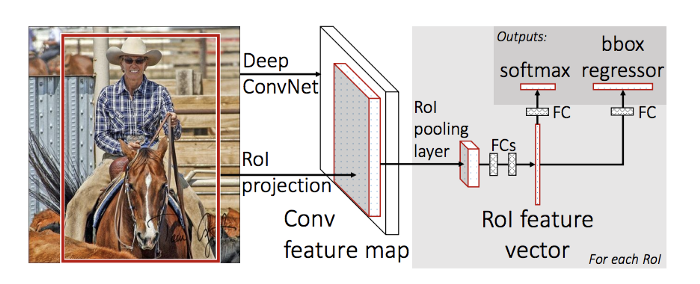
\includegraphics[scale=0.3]{gambar/fast-rcnn.png}
	\caption{Arsitektur \textit{Fast R-CNN} \citep{arch-fast-rcnn}}
	\label{fig:fast-rcnn}
\end{figure}

Alasan \textit{Fast R-CNN} lebih cepat daripada R-CNN adalah karena kita tidak perlu memasukkan 2000 \textit{region proposal} ke \textit{convolutional neural network} setiap saat. Sebagai gantinya, operasi konvolusi dilakukan hanya sekali per gambar dan \textit{feature map} dihasilkan operasi tersebut.

\subsection{\textit{Faster R-CNN}}
\label{subsec:faster-rcnn}

Pad kedua algoritma \textit{R-CNN} dan \textit{Fast R-CNN} menggunakan \textit{selective search} untuk mengetahui \textit{region proposal}. \textit{Selective search} sendiri memerlukan waktu yang cukup lama dalam penyelesain prosesnya sehingga mempengaruhi kinerja dari jaringan \citep{faster-rcnn}. Oleh karena itu, dibuatlah algoritma deteksi objek baru dengan menghilangkan algoritma \textit{selective search} dan memungkinkan jaringan mempelajari \textit{region proposal}.

Mirip dengan \textit{Fast R-CNN}, gambar dijadikann sebagai input ke jaringan konvolusi yang menyediakan \textit{convolusional feature map}. Disebabkan waktu eksekusi yang lama saat menggunakan algoritma \textit{selective search} pada \textit{feature map} untuk mengidentifikasi \textit{region proposal}, \textit{Faster R-CNN} menggunakan jaringan terpisah untuk memprediksi \textit{region proposal}. Jaringan terpisah ini dinamakan dengan \textit{Region Proposal Network (RPN)}, dimana \textit{RPN} berbagi \textit{full-image convolutional features} dengan jaringan deteksi yaitu \textit{Fast R-CNN}. \textit{Region proposal} yang diprediksi kemudian dibentuk kembali menggunakan \textit{ROI pooling layer} yang kemudian digunakan untuk mengklasifikasikan gambar di dalam \textit{region proposal} dan memprediksi nilai offset untuk \textit{bounding box}. Gambar \ref{fig:faster-rcnn} merupakan visualisasi dari proses deteksi objek menggunakan \textit{Faster R-CNN}. 

\begin{figure}[h]
	\centering
	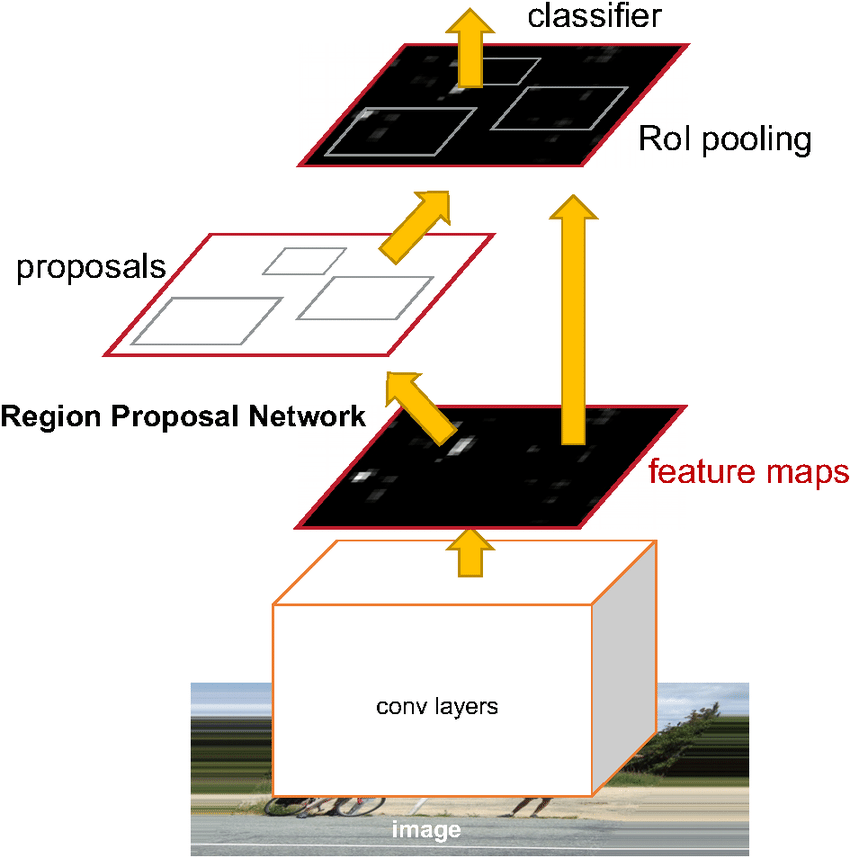
\includegraphics[scale=0.15]{gambar/arch-faster-rcnn.png}
	\caption{Gambaran Deteksi Objek pada \textit{Faster R-CNN} \citep{arch-faster-rcnn}}
	\label{fig:faster-rcnn}
\end{figure}

\subsection{\textit{Mask R-CNN}}
\label{subsec:mask-rcnn}

Mask R-CNN adalah Convolutional Neural Network (CNN) dan segmentasi citra termutakhir untuk saat ini. Varian Deep Neural Network ini mendeteksi objek dalam gambar dan menghasilkan \textit{mask} segmentasi berkualitas tinggi untuk setiap \textit{instance} \citep{mask-rcnn}. \textit{Mask R-CNN} dibangun menggunakan\textit{ Faster R-CNN} dimana \textit{Faster R-CNN} memiliki 2 \textit{output} untuk setiap objek, label kelas dan \textit{bounding box offset}. \textit{Mask R-CNN} adalah penambahan cabang ketiga yang mengeluarkan \textit{mask} objek seperti yang tertampil pada Gambar \ref{fig:arch-mask-rcnn}. \textit{output} \textit{mask} tambahan berbeda dari \textit{output} kelas dan \textit{bounding box}, yang membutuhkan ekstraksi tata letak spasial yang jauh lebih baik dari suatu objek.

\textit{Mask R-CNN} merupakan perpanjangan dari \textit{Faster R-CNN} dengan menambahkan cabang untuk memprediksi t\textit{mask} objek (\textit{Region of Interest}) secara paralel dengan cabang yang ada untuk pengenalan \textit{bounding box}. Satu keuntungan sederhana dari \textit{Mask R-CNN} dibandingkan \textit{Faster R-CNN} adalah kenyataan bahwa mudah untuk menggeneralisasi tugas lain seperti estimasi pose. Elemen kunci \textit{Mask R-CNN} adalah penyelarasan piksel-ke-piksel, yang merupakan bagian utama dari \textit{Fast/Faster R-CNN} yang hilang. \textit{Mask R-CNN} mengadopsi prosedur dua tahap yang sama dengan tahap pertama yang identik (yaitu \textit{RPN}). Pada tahap kedua, secara paralel untuk memprediksi kelas dan \textit{box offset}, Mask R-CNN juga mengeluarkan \textit{mask} biner untuk setiap \textit{RoI}. Ini berbeda dengan sistem terbaru, di mana klasifikasi bergantung pada prediksi \textit{mask}.

Mask R-CNN mudah diterapkan dan dilatih karena \textit{Faster R-CNN framework}, yang memfasilitasi berbagai desain arsitektur yang fleksibel. Selain itu, cabang \textit{mask} hanya menambahkan \textit{overhead} komputasi kecil, memungkinkan sistem dan eksperimen yang cepat.

\begin{figure}[H]
	\centering
	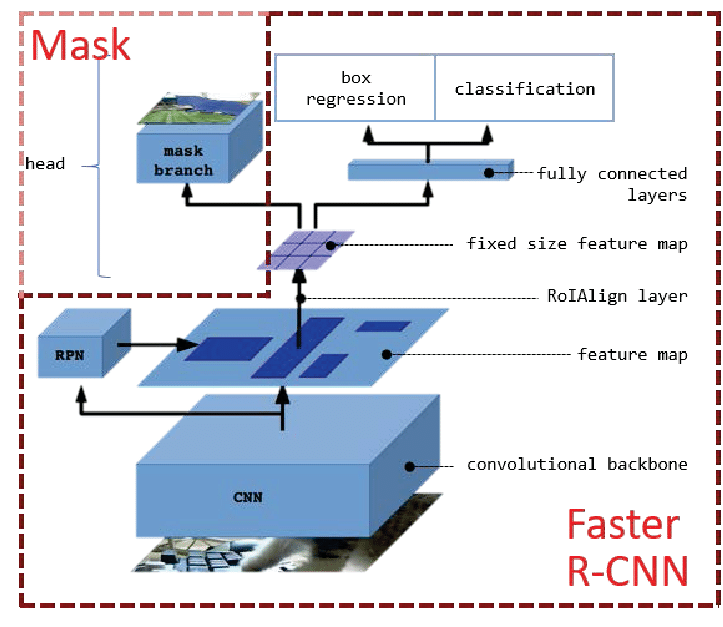
\includegraphics[scale=0.25]{gambar/arch-mask-rcnn.png}
	\caption{Struktur dari Arsitektur \textit{Mask R-CNN} \citep{arch-mask-rcnn}}
	\label{fig:arch-mask-rcnn}
\end{figure}

\subsection{\textit{Regional Proposal Network (RPN)}}
\label{subsec:rpn}

\textit{Regional Proposal} bermanfaat untuk mengetahui kemungkinan lokasi target pada gambar ke tingkat lebih akurat, yang dapat memastikan bahwa tingkat penarikan yang lebih tinggi dipertahankan ketika lebih sedikit jendela yang dipilih. Selanjutya jendela kandidat yang diperoleh dari proses tersebut, memiliki kualitas yang lebih tinggi dibandingkan dengan algoritma \textit{Sliding Window} pada umumnya. Algoritma \textit{Region Proposal} yang lebih umum digunakan adalah \textit{Selective Search} dan \textit{Bounding Box} \citep{rpn}.

\textit{Anchor boxes} merupakan satu kumpulan \textit{bounding box} dengan memiliki ukuran dan rasio aspek berbeda yang membentang di seluruh gambar \textit{input} untuk melatih \textit{region proposal network}. Pertama, akan digunakan beberapa lapisan awal dari jaringan yang telah dilatih sebelumnya untuk mengidentifikasi fitur yang menjanjikan dari gambar \textit{input}. Beberapa lapisan awal dari jaringan, akan belajar mendeteksi fitur umum, seperti tepi dan bintik warna pada gambar.

\textit{RPN} menggunakan klasifikasi dua kelas, yang hanya membedakan latar belakang dari objek, tetapi tidak memprediksi kelas objek. Misalkan setelah gambar dimasukkan dan mengalami serangkaian konvolusi dan \textit{pooling} di \textit{backbone network}, peta fitur ukuran M $\times$ N diperoleh, yang sesuai dengan membagi gambar asli menjadi area M $\times$ N. Pusat setiap area gambar asli diwakili oleh koordinat piksel pada peta fitur ini. 

\textit{RPN} digunakan untuk menentukan apakah \textit{anchor boxes} yang sesuai dengan setiap piksel, berisi target objek. Lapisan RPN harus belajar mengklasifikasikan \textit{anchor boxes} sebagai latar belakang atau latar depan, dan menghitung koefisien regresi untuk mengubah posisi, lebar, dan tinggi \textit{anchor boxes} latar depan.

\subsection{\textit{Region of Interest Align}}
\label{roialign}

\textit{Region of Interest Align}, atau \textit{RoIAlign}, adalah operasi untuk mengekstraksi peta fitur berukuran kecil dari setiap \textit{RoI} untuk deteksi dan segmentasi. Hal ini menghilangkan kuantisasi pada \textit{RoI Pool} serta menyelaraskan fitur yang diekstraksi dengan \textit{input} \citep{mask-rcnn}. Untuk menghindari kuantisasi batasan pada \textit{RoI}, \textit{RoIAlign} menggunakan interpolasi bilinear untuk menghitung nilai yang tepat dari fitur \textit{input} di empat lokasi sampel reguler di setiap \textit{bin RoI}, dan hasilnya kemudian dikumpulkan berdasarkan ninail maksimum atau rata-rata. 

Ide \textit{ROI Align} sangat sederhana yaitu dengan menghapus operasi kuantisasi, dan menggantinya dengan menggunakan metode interpolasi bilinear untuk mendapatkan nilai gambar pada piksel dengan koordinat \textit{floating point}, sehingga mengubah seluruh proses agregasi fitur menjadi operasi berkelanjutan. Perlu dicatat bahwa dalam operasi algoritma tertentu, \textit{ROI Align} tidak hanya melengkapi titik koordinat pada batas area kandidat, dan kemudian menggabungkan titik koordinat ini, tetapi mendesain ulang serangkaian proses yang lebih baik.

\subsection{Pejalan Kaki}
\label{subsec:pedestrian}

Definisi Pejalan kaki adalah orang yang melakukan aktifitas berjalan kaki dan merupakan salah satu unsur pengguna jalan. (Keputusan Direktur Jendral Perhubungan Darat : SK.43/AJ 007/DRJD/97). Pejalan kaki harus berjalan pada bagian jalan yang diperuntukan bagi pejalan kaki, atau pada bagian pejalan kaki, atau pada bagian jalan yang paling kiri apabila tidak terdapat bagian jalan yang diperuntukan bagi pejalan kaki (PP No. 43 , 1993)


\subsection{\textit{Zebra Cross}}
\label{subsec:zebracross}

\textit{Zebra cross} merupakan  fasilitas penyeberangan bagi pejalan kaki sebidang yang dilengkapi marka untuk memberi ketegasan/batas dalam melakukan lintasan. \textit{Zebra cross} dipasang dengan ketentuan sebagai berikut :
\begin{enumerate}[nolistsep]
	\item \textit{Zebra cross} harus dipasang pada arus lalu lintas, kecepatan lalu lintas, dan arus pejalan kaki yang relatif rendah.
	\item Lokasi penempatan \textit{zebra cross} harus memiliki jark pandang yang cukup, agar tundaan kendaranaan yang diakibatkan oleh penggunaan fasilitas penyebrangan masih dalam kondisi aman. 
\end{enumerate}

\subsection{ResNet-50}
\label{subsec:resnet50-definition}

ResNet50 adalah varian dari model ResNet yang memiliki 48 \textit{convolution layer} bersama dengan 1 \textit{MaxPool layer} dan 1 \textit{AveragePool layer}. ResNet-50 memiliki 3,8 x 10\^{}9 Operasi \textit{floating point}. Gambar \ref{fig:resnet50-arch} merupakan diagram proses dari arsitektur ResNet-50.
\begin{figure}[H]
	\centering
	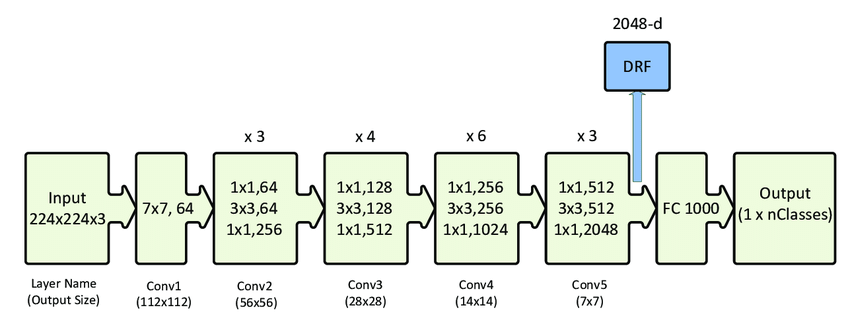
\includegraphics[scale=0.25]{gambar/resnet50-arch.png}
	\caption{Arsitektur ResNet-50 \citep{resnet50-arch}}
	\label{fig:resnet50-arch}
\end{figure}

\subsection{ResNet-101}
\label{subsec:resnet101-definition}

ResNet101 adalah varian dari model ResNet yang memiliki 99 \textit{convolution layer} bersama dengan 1 \textit{MaxPool layer} dan 1 \textit{AveragePool layer}. ResNet-101 memiliki 7,6 x 10\^{}9 Operasi \textit{floating point}. Gambar \ref{fig:resnet101-arch} merupakan diagram proses dari arsitektur ResNet-101.
\begin{figure}[H]
	\centering
	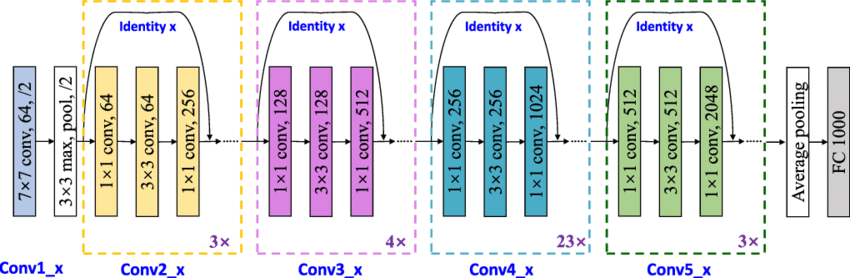
\includegraphics[scale=0.25]{gambar/resnet101-arch.png}
	\caption{Arsitektur ResNet-101 \citep{resnet101-arch}}
	\label{fig:resnet101-arch}
\end{figure}

\subsection{MobileNet-v1}
\label{subsec:mobilenetv1-definition}

MobileNets, merupakan salah satu arsitektur \textit{convolutional neural network} (CNN) yang dapat digunakan untuk mengatasi kebutuhan akan \textit{computing resource} berlebih. Seperti namanya, \textit{Mobile}, para peneliti dari Google membuat arsitektur CNN yang dapat digunakan untuk \textit{mobile device} atau ponsel \citep{mobilnet-def}. Perbedaan mendasar antara arsitektur MobileNet dan arsitektur CNN pada umumnya adalah penggunaan lapisan atau layer konvolusi dengan ketebalan filter yang sesuai dengan ketebalan dari \textit{input image}. MobileNet membagi konvolusi menjadi \textit{depthwise convolution} dan \textit{pointwise convolution}.

